\cite{Muon:WhitePaper}
\cite{Muon:Geer}
\cite{Muon:Collide}
\cite{Muon:Nature}
\cite{Muon:CERNCourier}
\cite{Muon:ProtonBeam}
\cite{Muon:Feasibility}
\cite{Muon:MICE}
\cite{Muon:PDG}

\subsubsection{Muons}

Muons ($\mu^-$) are elementary particles, and like electrons, are classified as leptons with spin $-\frac{1}{2}$ and charge of $-1$. However, muons have a mass of mμ = 105.7 $MeV/c^2$, which is about 200 times the mass of the electron (me = 0.511 $MeV/c^2$). Muons are also unstable particles with a mean lifetime of about 2.2$\mu s$. Its dominant decay process is given by:

\begin{equation}
    \mu^- \rightarrow e^- + \bar{\nu_e} + \nu_{\mu}
\end{equation}

where it decays into an electron, an anti-electron neutrino and a muon neutrino. The muon’s antiparticle, the anti-muon ($\mu^+$) decays into similar products: 

\begin{equation}
    \mu^+ \rightarrow e^+ + \nu_e + \bar{\nu_{\mu}}
\end{equation}    
 
where the products are simply the charge conjugates of the muon’s decay products.
 
\subsubsection{Muon Acceleration Program (MAP) and Muon Colliders}

With the recent interest in a lepton collider to be built as the next-generation collider after the LHC in CERN, there have been efforts within the scientific community to push forward the idea of a muon collider, compared to an electron-positron ($e^+ e^-$) collider such as the ILC or CLIC.
 
The United States Muon Accelerator Program (MAP) was set up in 2010 as a joint organisation between the Neutrino Factory and Muon Collider Collaboration (NFMCC) and the Muon Collider Task Force (MCTF) under the direction of the U.S. Department of Energy. Its goal is to develop the concepts and technologies required for the construction of Muon Colliders and Neutrino Factories for the physics community, which would hopefully further push the energy and technology frontier in particle physics research.
 
Muon colliders provide an interesting and attractive alternative when it comes to lepton colliders, especially in terms of the collider’s physics reach and potential development cost. This is mainly due to the muon’s aforementioned properties which allow higher efficiency while being able to achieve a higher-energy collider. Muon colliders are also a potentially unparalleled Neutrino Factory, capable of allowing physicists probe into Beyond Standard Model Physics in a world-class neutrino research facility. However, the concept of a muon collider is mainly plagued by its technical feasibility, as current goals of a muon collider would require more years of research and development into innovative, new technology that currently have not necessarily been shown to be demonstrable at a laboratory scale.
 
\subsubsection{Physics Reach/Goals}
 
The current proposal put forth for a muon collider would be a circular multi-TeV collider that could reach centre-of-mass energies of 4 TeV, with a luminosity goal of $10^{34}$ \textemdash $10^{35} cm^{-2} s^{-1}$. The diameter of such a collider would be approximately 2-3 km, which would fit easily within the footprint of the Fermilab site. The Muon Collider’s early stages would also see it serve as a Neutrino Factory, which would provide the physics community with a world-class neutrino research program.
 
The current concept to such a monumental project would be a staged approach to the construction, where at each stage, the facility will have a unique and important physics reach with increasing complexity; this begins with a Neutrino Factory facility (nuSTORM, nuMAX and nuMAX+, with increasing intensity), followed by a Higgs Factory capable of producing up to 13,500 high resolution Higgs events a year, and culminating in a multi-TeV muon collider.
 
\subsubsection{Neutrino Physics}
 
Muon colliders provide a promising source of neutrinos needed to produce an intense neutrino beam for research. Previous laboratory sources of neutrinos only produce one dominant flavour of neutrinos. Charged kaons and pions were allowed to decay in long, straight decay channels into muon neutrinos, with a small percentage of three-body decays that produce electron neutrinos. This small percentage of electron neutrinos was considered to be an undesirable contamination in the otherwise “pure” neutrino beam. Due to the muon’s dominant decay into two different flavours of neutrinos, it is certain that the decay produces 50\% of each flavour, eliminating the contamination problem. Hence, they represent a new and better way of producing an intense neutrino beam required for high quality neutrino research.
 
\begin{figure}[!htb]
\centering
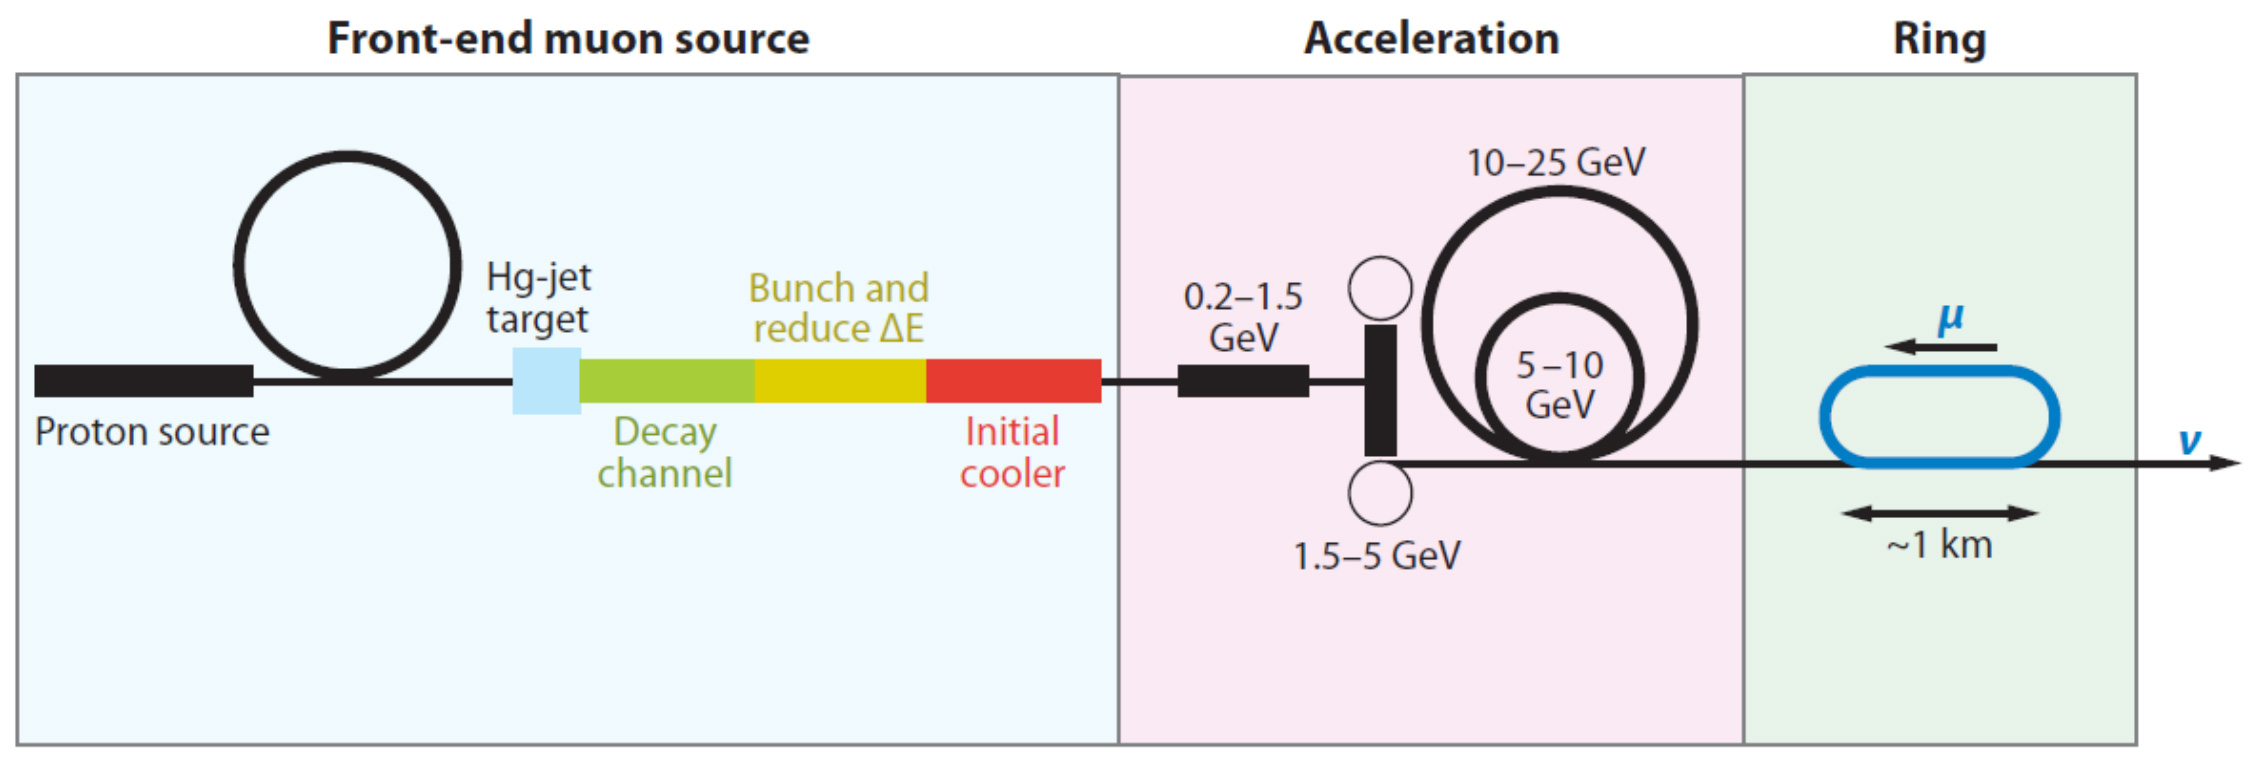
\includegraphics[width=1\textwidth,natwidth=2254,natheight=772]{Muon_Neutrino.jpg}
\caption{Schematic Diagram of the Neutrino Factory Planned for a Muon Collider}
\end{figure}
 
Protons are fired at a dense mercury (Hg) target, where the resulting collision produces $\pi \pm$ that are allowed to decay and into daughter muons. These daughter muons then undergo phase rotation before being cooled for acceleration into a muon storage ring.
 
\subsubsection{Multi-TeV Collider}
 
When working with charged particles in colliders, the main efficiency concern would be energy loss through synchrotron radiation. The biggest difference between a muon and an electron is their masses; therefore, this relation is particularly important when comparing the differences between an electron and a muon collider.
 
Compared to a linear $e^+ e^-$ collider, a muon collider would instead be a circular collider, much like the LHC. This is because unlike electrons, muons suffer much less synchrotron radiation due to its larger mass. Since the ratio of masses $\frac{m_{\mu}}{m_e}$ is about 200, $\frac{m_{\mu}}{m_e}^4 = 2 \times 10^9$ would mean that these radiation effects will be greatly reduced. Hence, a muon collider would enjoy all the benefits that come from circular colliders, such as multiple circulations, multi-turn collisions and multiple interaction points that increase events observed, while also benefitting from the clean collision environment as provided from a lepton collider. These greatly increase the overall efficiency of the collider, and reduce the overall power consumption of a muon collider compared to that of a linear $e^+ e^-$ collider.
 
The ability of a muon collider to reach energy levels beyond that of even CLIC (which has a maximum energy level of $\sim$3 TeV) is also due to the large mass of the muon. The large mass of the muon, compared to the electron, means that it is also easier to accelerate muons to higher energies. Added on to the fact that muons suffer less from synchrotron radiation, means that a muon collider is able to reach energies beyond the feasibility range of a linear lepton collider, in terms of a feasible length and size.
 
\subsubsection{Higgs Factory/Measurement}
 
One of the goals that the physics community is hoping that the next collider would adequately achieve would be precise measurements of the Higgs particle, recently discovered at the LHC in 2012.  A muon collider would be a great candidate to fulfil that goal as it couples much more strongly to the Higgs field (and hence the boson) due to its larger mass. In fact, as the mass-dependent Higgs coupling is proportional to the mass of the lepton, the coupling of the Higgs to a muon is approximately $\frac{m}{m_e}^2 = 4 \times 10^4$ times larger than that of an electron’s.
 
As the muon collider would be a circular collider, this also allows multiple interaction points which increase the event rate and allow multiple simultaneous experiments. The reduction in synchrotron losses also means that a muon collider can have more precise beam-energy constraints and a sharper distribution for signals that allow for greater precision in mass and width measurements.

\subsubsection{Technical Feasibility}
 
The main challenge of muon colliders lies in the fact that compared to other more robust and proposals such as the ILC, it would require much more advanced technology that are not necessarily demonstrable in a laboratory setting as of now. To achieve the ultimate goal of a multi-TeV collider, it would require a powerful proton linac and target station, the ability to cool muons down to a narrow, cold beam, and finally a suitable acceleration scheme for rapid beam acceleration.
 
To achieve the high-power proton linac required for muon production, the Mercury Intense Target (MERIT) Experiment was set up to develop the technology required for a target station capable of handling  more than 4MW of power. Recent results from MERIT have shown proof of a free Hg-jet target technology that is capable of handling the required proton beam power without dispersion of jet target due to shock and/or vaporisation, and without damping due to the strong magnetic field from the capture solenoid ($\sim$20T).
 
However, the biggest technological challenge lies in muon cooling and acceleration. As the muons are produced from decay processes after smashing protons into a dense Hg target, the energy spread of muons is significantly large. The challenge is to be able to cool these muons down to a size small enough so that they form an extremely narrow cold beam suitable for acceleration. Moreover, given the short lifetime of the muon, a rapid acceleration system is required to accelerate these cooled muons before they decay.
 
To tackle these issues, the International Muon Ionisation Cooling Experiment (MICE) was set up to develop novel and innovative technologies in ionisation cooling in order to achieve the 6-orders-of-magnitude cooling channel required.
 
\begin{figure}[!htb]
\centering
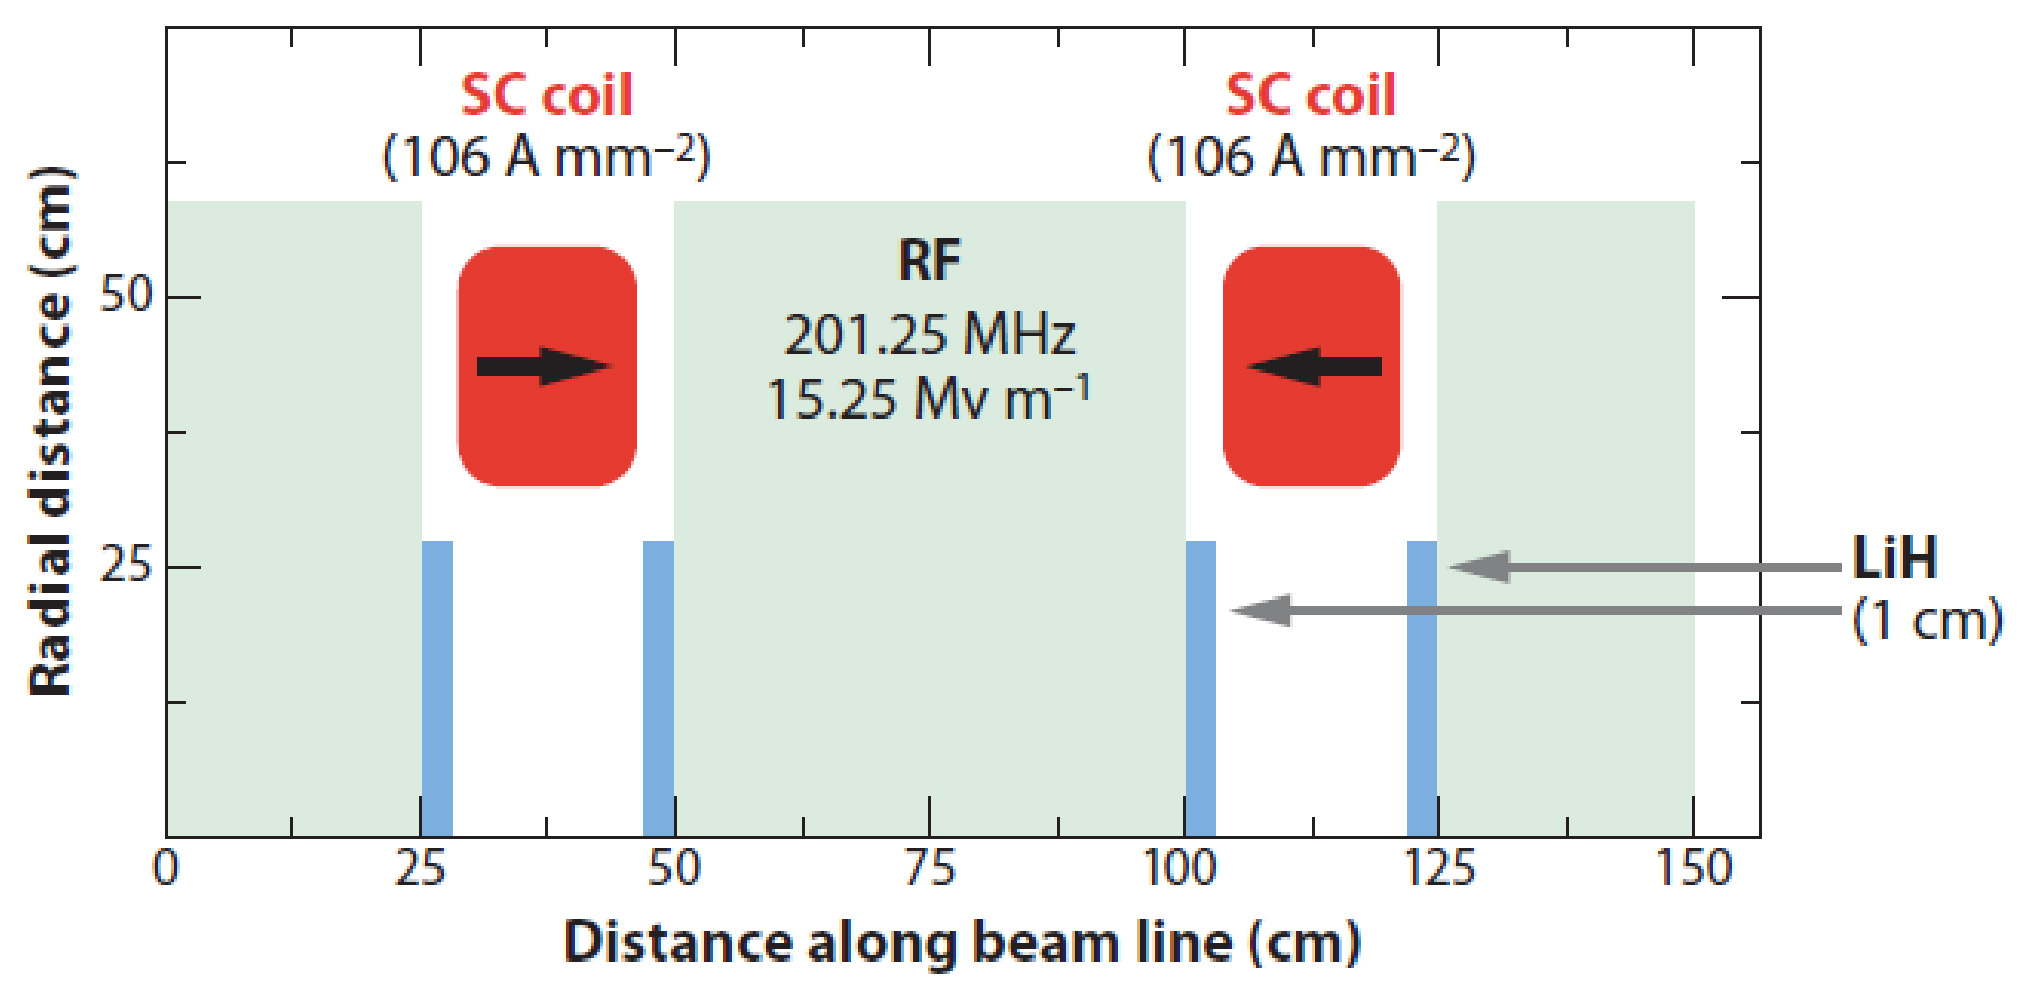
\includegraphics[width=0.7\textwidth,natwidth=2026,natheight=1000]{Muon_Cooling.jpg}
\caption{Schematic Diagram of the Ionisation Cooling Process}
\end{figure}
 
The rate at which normalised transverse emittance $\epsilon$ is lost as muons of energy $E$ travel through a material with radiation length $L_R$ is given by:
 
\begin{equation}
    \frac{d \epsilon}{ds} = - \frac{dE}{ds} \frac{\epsilon}{E} + \frac{\beta_{\perp} (0.014)^2}{2 E m_{\mu} L_R}
\end{equation}
 
where $\beta_{\perp}$ is the betatron function (which represents the focusing strength at the absorber), $m$ is the mass of the muon and $\frac{dE}{ds}$ is the energy loss through ionisation loss. In order to reduce their longitudinal and transverse momenta, the muons are passed through a series of absorbers of low Z (with large $L_R$) such as lithium hydride and to use strong solenoids to focus the beam (to reduce $\beta_{\perp}$). However, in order to maintain the muon’s longitudinal momentum (to form a muon beam), it goes through a series of radio-frequency (RF) cavities to re-accelerate the muons longitudinally. This reduces the overall transverse emittance of the muons.
 
According to the 2013 White Paper submitted by MAP, the first results for transverse cooling are expected from MICE by 2015 for one cooling station and no re-acceleration of muons, while the results from a full cooling cell with acceleration is expected by 2019. However, results from ionisation cooling demonstrated at a reasonable intensity of muons are expected by 2022. As observed, the technology required for muon colliders are still not demonstrable, and while great strides have been made, it is nowhere as mature or as ready as the technology needed for the ILC, or even CLIC.
 
\subsubsection{Development Cost}
 
As a muon collider still requires many years of R\&D before a robust proposal or design report can be achieved, the current development cost estimates are relatively unknown. However, given the knowledge that a muon collider would be much more compact and more efficient in terms of power consumption, it is a reasonable estimate that the cost of construction of a muon collider might be much more economical as compared to a linear $e^+ e^-$ collider. Figure \ref{Muon:Layout} shows how the muon collider would easily fit within the Fermilab site.

\begin{figure}[!htb]
\centering
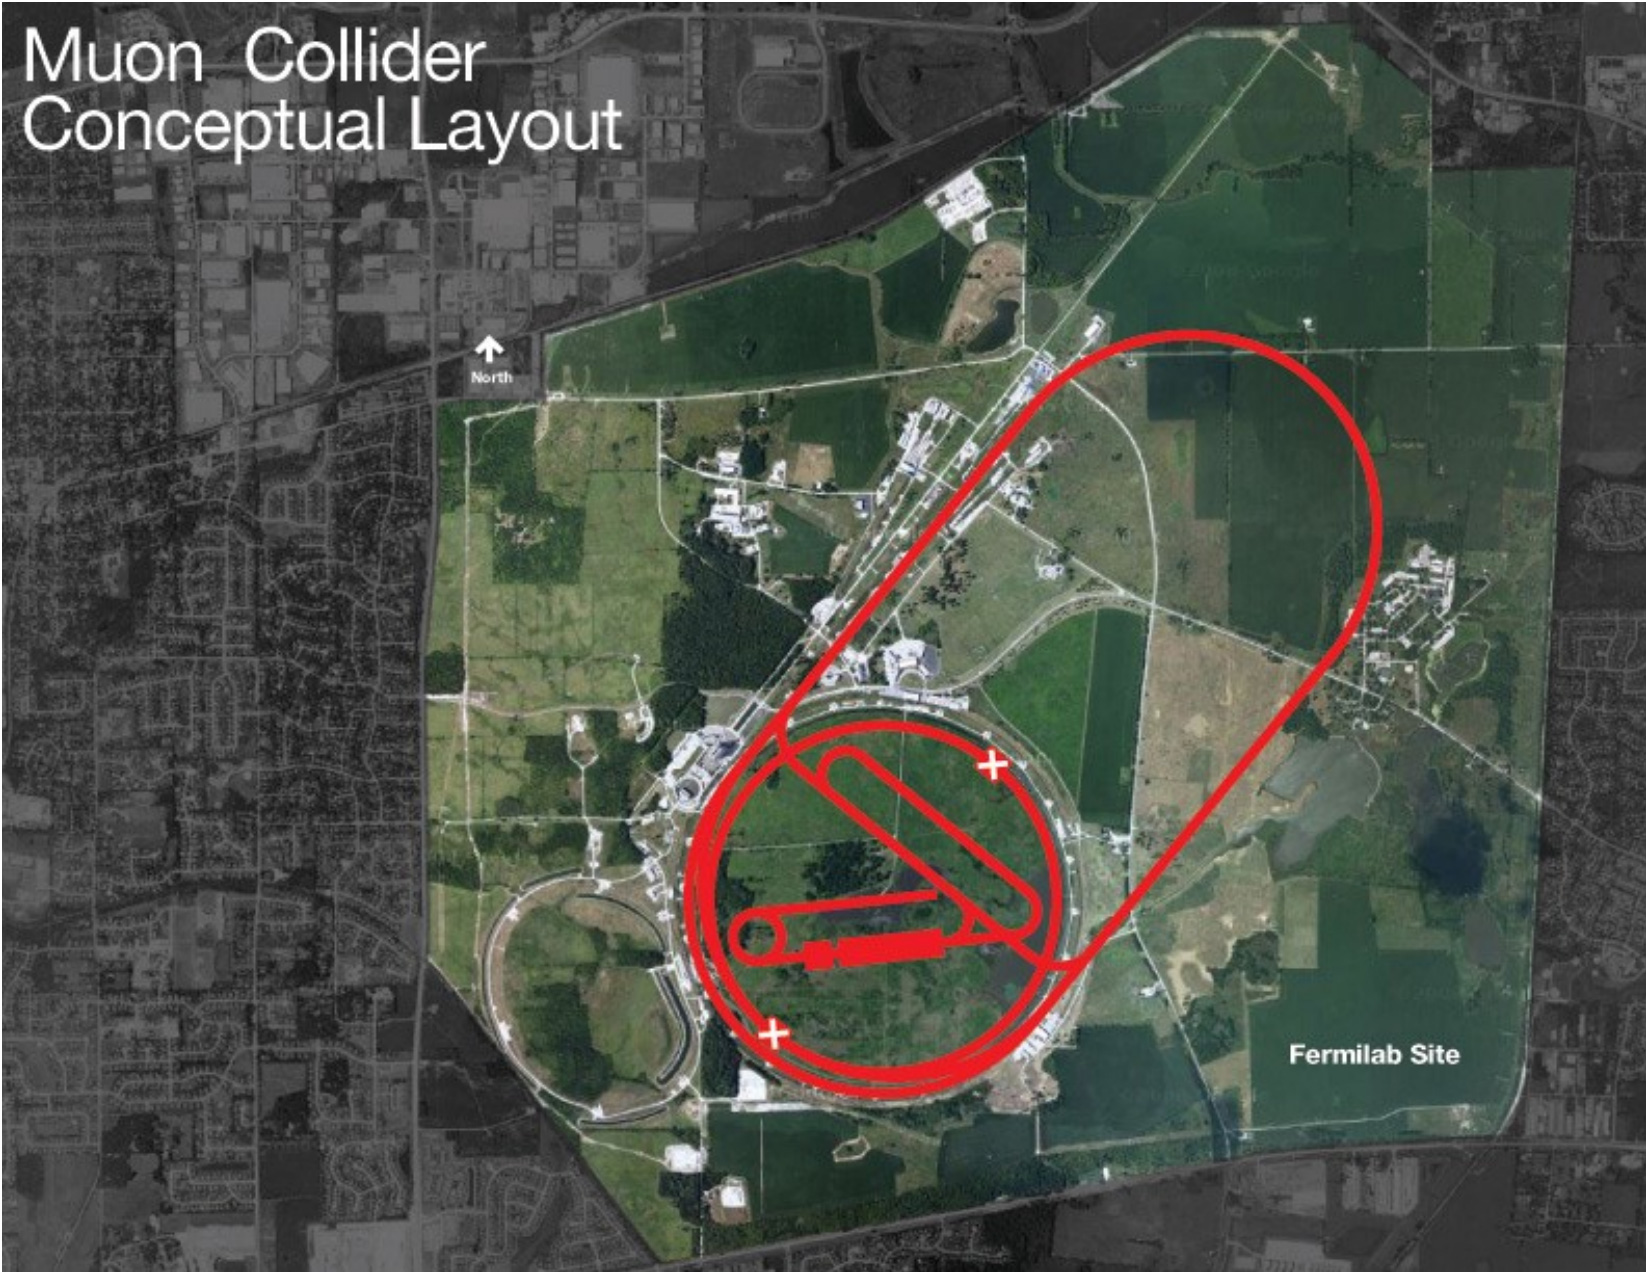
\includegraphics[width=0.6\textwidth,natwidth=1646,natheight=1272]{Muon_Layout.jpg}
\caption{Muon Collider Layout at Fermilab}
\label{Muon:Layout}
\end{figure}
 
The staged approach to building the entire collider would hopefully reduce the required investment at each stage, further reducing the overall cost of the project. This is of paramount importance as the current site of the collider is in the United States, and given the current economic situation, the United States has been unwilling to host a large project like the ILC, let alone a relatively untested muon collider. However, given the years needed to conduct the necessary research, the economic situation of the U.S. may have drastic changes over the decades that are hard to predict.